% \documentclass[a4paper, 12pt]{article}
\documentclass[twoside,a4,english,11pt]{book}
\usepackage[margin=1in]{geometry}
% \documentclass[a4paper, twoside=semi, BCOR=5mm, 12pt]{scrbook}
% \usepackage{cleveref}
% \DeclareMathSizes{12}{20}{14}{10}

% \usepackage[toc]{glossaries}
% \renewcommand*{\glsgroupskip}{}
% \renewcommand*{\glsseeformat}[3][\seename]{(\xmakefirstuc{#1}\glsseelist{#2}.)}

% \titlehead{
% {\Large Unseen University \hfill SS~2002\\}
%  Higher Analytical Institute\\
%  Mythological Rd\\
%  34567 Etherworld
% }

\pagestyle{plain}

\usepackage[utf8x]{inputenc}
\usepackage[british]{babel}

% \parindent 1cm
% \parskip 0.2cm
% \topmargin 0.2cm
% \oddsidemargin 1cm
% \evensidemargin 0.5cm
% \textwidth 15cm
% \textheight 21cm

% ******************************************************************************
% B5 book boxing
% ******************************************************************************

% \addtolength{\oddsidemargin}{-0.2345679in} % magic number = 1 - 1/0.81 
% \addtolength{\oddsidemargin}{−0,19047619in} % magic number = 1 - 1/0.81 
% \addtolength{\evensidemargin}{−0,19047619in} % magic number = 1 - 1/0.81 
% \addtolength{\evensidemargin}{-0.2345679in}% see documentation scale package 
% \addtolength{\topmargin}{-0.2345679in} % for explanation 
% \mag=840 % basic TeX command for 81% scaling 
% \usepackage[b5paper]{geometry}
% \usepackage[pdflatex,cam,a4,center,frame]{crop}

% \usepackage[pdflatex, b5, center, frame]{crop}
% % \usepackage{showframe}  

% \usepackage{setspace}
% \onehalfspace
% \singlespace

% \usepackage[scaled]{helvet}
% \usepackage{sectsty}
% \usepackage{amsmath,amssymb,amsfonts}

% \usepackage[OT1]{fontenc}
% \usepackage{iwona}
% \usepackage{tgpagella}
% \usepackage{pandora}

% \usepackage[T1]{fontenc}
% \usepackage{efont,mathesf}
% \renewcommand*\oldstylenums[1]{{\fontfamily{esfod}\selectfont#1}}


\usepackage[T1]{fontenc}
% \usepackage{libertine}
% \usepackage[seriftt]{lucidabr}
% \usepackage[scaled=0.8]{beramono}
\usepackage{amsfonts}


\usepackage{graphicx}
\usepackage{lettrine}

\usepackage[unicode=false,
 bookmarks=true,bookmarksnumbered=true,bookmarksopen=true,
 breaklinks=true, backref=false, colorlinks=false]
 {hyperref}
\hypersetup{
    unicode=true,          % non-Latin characters in Acrobat’s bookmarks
    pdftoolbar=true,        % show Acrobat’s toolbar?
    pdfmenubar=true,        % show Acrobat’s menu?
    pdffitwindow=false,     % window fit to page when opened
    pdfstartview={FitV},    % fits the width of the page to the window
    pdfsubject={Parallel performance analysis},   % subject of the document
%     pdfcreator={Creator},   % creator of the document
%     pdfproducer={Producer}, % producer of the document    
    pdfnewwindow=true,      % links in new window
    pdftitle={ClusteringSuite Manual},    % title
    pdfauthor={Juan Gonzalez Garcia},     % author
    pdfkeywords={high performance computing, parallel applications, performance analysis, automatic analysis,cluster analysis, sequence analysis, data mining}, % list of keywords
}

\usepackage[numbers]{natbib}
\usepackage{bibentry}

% \newcommand{\ignore}[1]{}
% \newcommand{\nobibentry}[1]{{\let\nocite\ignore\bibentry{#1}}}
% % apsrev entries in the text need definitions of these commands
% \newcommand{\bibfnamefont}[1]{#1}
% \newcommand{\bibnamefont}[1]{#1}

% \usepackage{floatrow}
\usepackage{subfig}
% \usepackage{subcaption}
% \usepackage{subfigure}

% \usepackage{boxedminipage}
\usepackage{tikz}
% \usepackage{caption}

% \usepackage{xcolor}
% \usepackage{fancybox}

\usepackage{lipsum}
\usepackage{multicol}

% \usepackage{multirow}
% \usepackage{colortbl}

% \usepackage{makecell}

% \newcommand{\goodgap}{%
% \hspace{\subfigtopskip}%
% \hspace{\subfigbottomskip}}

% \usepackage[stretch=10]{microtype}

% \usepackage{float}

\usepackage{amsmath}

\usepackage{algorithmic}
\usepackage{algorithm2e}

% \usepackage{afterpage}
% \usepackage{pdflscape}
\usepackage{rotating}

% \usepackage{graphicx}
\usepackage{array}

\usepackage{booktabs}
\usepackage{arydshln}
\usepackage{xcolor}   % http://ctan.org/pkg/xcolor
\usepackage{colortbl} % http://ctan.org/pkg/colortbl
% \usepackage{dcolumn}

\usepackage{fancyvrb}
\usepackage{threeparttable}

% \usepackage{varwidth}

\usepackage[toc,page,header]{appendix}
\usepackage{minitoc}

\usepackage{floatrow}

% \usepackage{pdfpages}
\urlstyle{leostyle}

\makeatletter
\def\url@leostyle{
  \@ifundefined{selectfont}{\def\UrlFont{\sf}}{\def\UrlFont{\small\ttfamily}}}
\usepackage{babel}
\makeatother

% \long\def\greybox#1{%
%     \newbox\contentbox%
%     \newbox\bkgdbox%
%     \setbox\contentbox\hbox to \hsize{%
%         \vtop{
%             \kern\columnsep
%             \hbox to \hsize{%
%                 \kern\columnsep%
%                 \advance\hsize by -2\columnsep%
%                 \setlength{\textwidth}{\hsize}%
%                 \vbox{
%                     \parskip=\baselineskip
%                     \parindent=0bp
%                     #1
%                 }%
%                 \kern\columnsep%
%             }%
%             \kern\columnsep%
%         }%
%     }%
%     \setbox\bkgdbox\vbox{
%         \pdfliteral{0.85 0.85 0.85 rg}
%         \hrule width  \wd\contentbox %
%                height \ht\contentbox %
%                depth  \dp\contentbox
%         \pdfliteral{0 0 0 rg}
%     }%
%     \wd\bkgdbox=0bp%
%     \vbox{
%       \hbox to \hsize{
%         \box
%         \bkgdbox
%         \box
%         \contentbox
%       }
%     }%
%     \vskip\baselineskip%
% }

\definecolor{shade}{HTML}{D4D7FE}
% \definecolor{figureshade}{HTML}{D4D7FE}
% \definecolor{figureshade}{gray}{0.80}
\definecolor{figureshade}{gray}{.7}

\long\def\innercite#1
{
  \vspace{10pt}
  \noindent
  \begin{tikzpicture}
    \node [fill=shade,rounded corners=5pt]
    {
      \begin{tabular}{p{.03\columnwidth}p{.89\columnwidth}}
        ~\cite{#1} & ~\bibentry{#1}
      \end{tabular}
    };
  \end{tikzpicture}
  \vspace{-10pt}
}
% \long\def\innercite#1
% {
% \begin{tabular}{p{.03\columnwidth}p{.89\columnwidth}}
% ~\cite{#1} & ~\bibentry{#1}
% \end{tabular}
% }

% \newcommand{\floatbox}[1]
% {
% {
%   \vspace{10pt}
%   \noindent
%   \begin{tikzpicture}
%     \node [fill=figureshade,rounded corners=5pt]
%     {
%       #1
%     };
%   \end{tikzpicture}
%   \vspace{-10pt}
% }
% }

% ROTATED COLUMN HEADER
\newcommand\rotcolhead[1]{\begin{sideways}\textbf{\makecell[l]{#1}}\end{sideways}} 

% REGULAR COLUMN HEADER WITH BREAKLINES
\newcommand\colhead[1]{\textbf{\makecell[r]{#1}}} 


\newcommand\myVSpace[1][10pt]{\rule[\normalbaselineskip]{0pt}{#1}}

\def\verbatimboxed#1
{
  \begingroup
  \def\verbatim@processline
  {
    {
      \setbox0=\hbox{\the\verbatim@line}
      \hsize=\wd0
      \the\verbatim@line\par
    }
  }
  
  \setbox0=\vbox{
    \parskip=0pt\topsep=0pt\partopsep=0pt\verbatiminput{#1}
  }%
  
  \begin{center}\fbox{\box0}\end{center}%
  \endgroup
}

\newcolumntype{d}[1]{D{.}{\cdot}{#1}}

\newcommand{\ra}[1]{\renewcommand{\arraystretch}{#1}}

\newcolumntype{*}{>{\global\let\currentrowstyle\relax}}
\newcolumntype{^}{>{\currentrowstyle}}
\newcommand{\rowstyle}[1]{\gdef\currentrowstyle{#1}%
  #1\ignorespaces
}

\colorlet{tableheadcolor}{gray!25} % Table header colour = 25% gray
\newcommand{\headcol}{\rowcolor{tableheadcolor}} 

\newcommand{\rowcol}{\rowcolor{tablerowcolor}} %
    % Command \topline consists of a (slightly modified) \toprule followed by a \heavyrule rule of colour tableheadcolor (hence, 2 separate rules)
\newcommand{\topline}{\arrayrulecolor{black}\specialrule{0.1em}{\abovetopsep}{0pt}%
            \arrayrulecolor{tableheadcolor}\specialrule{\belowrulesep}{0pt}{0pt}%
            \arrayrulecolor{black}}
    % Command \midline consists of 3 rules (top colour tableheadcolor, middle colour black, bottom colour white)
\newcommand{\midline}{\arrayrulecolor{tableheadcolor}\specialrule{\aboverulesep}{0pt}{0pt}%
            \arrayrulecolor{black}\specialrule{\lightrulewidth}{0pt}{0pt}%
            \arrayrulecolor{white}\specialrule{\belowrulesep}{0pt}{0pt}%
            \arrayrulecolor{black}}
    % Command \rowmidlinecw consists of 3 rules (top colour tablerowcolor, middle colour black, bottom colour white)
\newcommand{\rowmidlinecw}{\arrayrulecolor{tablerowcolor}\specialrule{\aboverulesep}{0pt}{0pt}%
            \arrayrulecolor{black}\specialrule{\lightrulewidth}{0pt}{0pt}%
            \arrayrulecolor{white}\specialrule{\belowrulesep}{0pt}{0pt}%
            \arrayrulecolor{black}}
    % Command \rowmidlinewc consists of 3 rules (top colour white, middle colour black, bottom colour tablerowcolor)
\newcommand{\rowmidlinewc}{\arrayrulecolor{white}\specialrule{\aboverulesep}{0pt}{0pt}%
            \arrayrulecolor{black}\specialrule{\lightrulewidth}{0pt}{0pt}%
            \arrayrulecolor{tablerowcolor}\specialrule{\belowrulesep}{0pt}{0pt}%
            \arrayrulecolor{black}}
    % Command \rowmidlinew consists of 1 white rule
\newcommand{\rowmidlinew}{\arrayrulecolor{white}\specialrule{\aboverulesep}{0pt}{0pt}%
            \arrayrulecolor{black}}
    % Command \rowmidlinec consists of 1 tablerowcolor rule
\newcommand{\rowmidlinec}{\arrayrulecolor{tablerowcolor}\specialrule{\aboverulesep}{0pt}{0pt}%
            \arrayrulecolor{black}}
    % Command \bottomline consists of 2 rules (top colour
\newcommand{\bottomline}{\arrayrulecolor{white}\specialrule{\aboverulesep}{0pt}{0pt}%
            \arrayrulecolor{black}\specialrule{\heavyrulewidth}{0pt}{\belowbottomsep}}%
\newcommand{\bottomlinec}{\arrayrulecolor{tablerowcolor}\specialrule{\aboverulesep}{0pt}{0pt}%
            \arrayrulecolor{black}\specialrule{\heavyrulewidth}{0pt}{\belowbottomsep}}%

\newcommand{\mypow}[2]{\textnormal{#1}\ensuremath{\times\textrm{10}^\textrm{{#2}}}}
\newcommand{\sps}[1]{\ensuremath{^{\textrm{#1}}}}
\newcommand{\sbs}[1]{\ensuremath{_{\textrm{#1}}}}


\begin{document}

\graphicspath{{figures/}}

\title{\sf {ClusteringSuite} Introductory Manual
\author{
tools@bsc.es}}

\maketitle

\chapter{Quick start guide}

The \textsf{ClusteringSuite} is the software package that includes the cluster
analysis tool developed at the Barcelona Supercomputing Center Tools Team. 
It is composed by a set of binaries and libraries implemented in C and C++.
The main tool included in this package is \texttt{BurstClustering}, which
performs the cluster analysis of Paraver traces (see section~\ref{sec:about_tools}).

As a short summary, the cluster analysis tool finds groups in the different
computations (\emph{CPU bursts}, i.e. regions between call to the parallel
runtime) a parallel application performs. To characterize these bursts we can
use any information gathered in the input trace. In almost all cases we use the
information provided by the Performance Hardware Counters.

In this first chapter of this manual we detail the contents of the package
as well as we guide how to run the first cluster analysis, following the
example distributed with the \textsf{ClusteringSuite} package.

\section{\textsf{ClusteringSuite} package}

The package is distributed in compressed tar format (e.g., clusteringsuite.tar.gz).
To unpack it, execute from the desired target directory the following command line :

\begin{figure}[!h]
  
  
\begin{tikzpicture}
  \node [fill=figureshade,rounded corners=5pt, align=center]
  {

  \begin{minipage}{.8\textwidth}
  \centering
  \texttt{> tar xvfz clusteringsuite.tar.gz}
  \end{minipage}
  };
  \end{tikzpicture}
\end{figure}

The unpacking process will create different directories on the current directory
(see table~\ref{tab:package_description}). We suggest adding the 
\texttt{<clusteringsuite\_dir>/bin} directory to your PATH environment variable,
so as to easily access to the tools included in the package.

\begin{table}[!ht]
\centering
  
  \caption{Package contents description}
  \label{tab:package_description}
  
  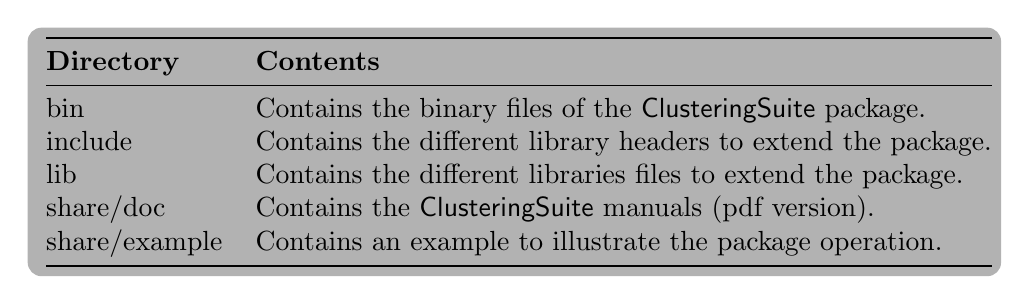
\begin{tikzpicture}
  \node [fill=figureshade,rounded corners=5pt]
  {
  
    \vspace{10pt}
  
    \begin{tabular}{@{}ll@{}}
    \toprule
    {\bf Directory}     & {\bf Contents} \\
    \midrule
    bin           & Contains the binary files of the \textsf{ClusteringSuite} package.\\
    % \hline
    include       & Contains the different library headers to extend the package.\\
    % \hline
    lib           & Contains the different libraries files to extend the package.\\
    % \hline
    share/doc     & Contains the \textsf{ClusteringSuite} manuals (pdf version).\\
    % \hline
    share/example & Contains an example to illustrate the package operation.\\
    \bottomrule
    \end{tabular}
  };
  \end{tikzpicture}

\end{table}

\section{Running the cluster analysis example}

As listed in Table~\ref{tab:package_description}, in the \textsf{ClusteringSuite}
package we include an example to illustrate the basic operation of 
\texttt{BurstClustering}, the main analysis tool included in the package.
If you move into the directory \texttt{share/example} you will find the
files 6 listed in Table~\ref{tab:example_directory}.

\begin{table}
  \centering
  
  \caption{Contents of \texttt{share/example} directory}
  \label{tab:example_directory}
  
  \begin{tikzpicture}
  \node [fill=figureshade,rounded corners=5pt]
  {
  
  \vspace{10pt}
  
%   \ra{1.3}
  
  \begin{tabular}{@{}*l^p{6cm}@{}}
\toprule
{\bf File}     & {\bf Description} \\
\midrule
README                & Text file with the same instructions of this section. \\
% \hline
cluster\_explained.xml  & Clustering configuration XML file with brief descriptions about the different fields.\\
% \hline
cluster.xml            & Same clustering configuration XML file as the previous one, without the descriptions. \\
% \hline
su3.lat256\_2it.16tasks.[prv|pcf|row] & Paraver trace to be used in the example.\\
\bottomrule
  
  \end{tabular}
  
  };
  \end{tikzpicture}
  
\end{table}

The XML configuration files provided use Completed Instructions hardware counter,
PAPI\_TOT\_INS in PAPI terminology, and Instructions Per Cycle (IPC), derived using 
PAPI\_TOT\_INS / PAPI\_TOT\_CYC counters, as clustering parameters. It sets a 
duration filter of 1000$\mu s$ and a Completed Instructions filter of \mypow{3}{8}. 
It configures the extrapolation of all the counters present in the input trace
and defines a single output plot combining the two clustering metrics, depicting
the raw values.

The input trace provided is a two iteration chop from an execution with 16 tasks
of \textsf{SU3\_AHiggs}, a lattice quantum chromodynamics code, part of the PRACE
benchmark suite~\footnote{\url{http://www.prace-ri.eu/ueabs\#QCD} - Kernel B}.

\subsection{Executing \texttt{BurstClustering} tool}

You can execute the cluster analysis with the provided XMLs without modification
running the following command:

\begin{figure}[!h]
  
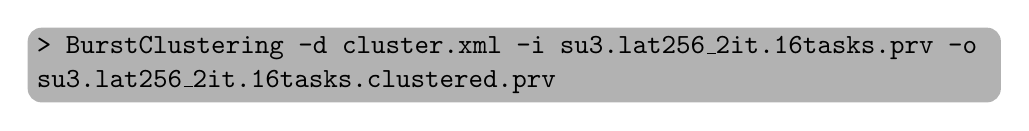
\begin{tikzpicture}
\node [fill=figureshade,rounded corners=5pt]
{

\begin{minipage}{1\textwidth}
% \fontsize{9}{10}
\texttt{> BurstClustering -d cluster.xml -i su3.lat256\_2it.16tasks.prv -o su3.lat256\_2it.16tasks.clustered.prv}
\end{minipage}
};
\end{tikzpicture}

\end{figure}


As a result of this execution, the 'BurstClustering' tool will detect 14
clusters in the input data.

\subsection{\texttt{BurstClustering} outputs}

The \texttt{BurstClustering} tool will generate the following outputs:

\begin{itemize}

  \item \texttt{su3.lat256\_2it.16tasks.clustered.[prv|pcf|row]}: a Paraver
  trace with clusters information. You can load this trace in Paraver, and use
  the clustering configuration files to analyse the clusters behaviour with the
  time context. In the default distribution of Paraver, these configuration
  files are installed in the directory \texttt{\${PARAVER\_HOME}/cfgs/clustering}.
 
  \item \texttt{su3.lat256\_2it.16tasks.clustered.clusters\_info.csv}: a CSV file
  with clusters statistics, including the aggregated duration of each cluster,
  the average duration of the bursts of each cluster, and the average values of
  the cluster parameters and the extrapolation parameters. You can import this
  file to a regular spreadsheet application to analyse the clusters behaviour
  as a group.
 
  \item \texttt{su3.lat256\_2it.16tasks.clustered.IPC.PAPI\_TOT\_INS.gnuplot}: a
  GNUPlot script to observe the resulting clusters in a 2D scatter plot. To
  visualize it, execute:

  \begin{figure}[!h]
  
  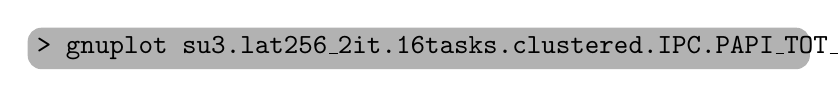
\begin{tikzpicture}
  \node [fill=figureshade,rounded corners=5pt]
  {

  \begin{minipage}{.8\textwidth}
  \texttt{> gnuplot su3.lat256\_2it.16tasks.clustered.IPC.PAPI\_TOT\_INS.gnuplot}
  \end{minipage}
  };
  \end{tikzpicture}

  \end{figure}

  \item \texttt{su3.lat256\_2it.16tasks.clustered.DATA.csv}: a CSV file with the 
  characterization of each burst read from the input trace, including its 
  clustering and extrapolation parameters value, as well as the timestamps and
  cluster id assigned. This file is used by the GNUPlot script, but you can
  also load it in a spreadsheet or any other software to analyse the different
  CPU burst instances that took part in the cluster analysis process.
 
\end{itemize}

% This document is intended as a brief manual of \texttt{BurstClustering}, the binary that encapsulates the cluster analysis
% features offered.

\section{About \textsf{Extrae} and \textsf{Paraver}}

\textsf{Extrae} and \textsf{Paraver} are two of the core tools of the BSC 
Performance Analysis Tools ecosystem.

\textsf{Extrae} is a dynamic instrumentation package to trace programs compiled
and run with the shared memory model (like OpenMP and pthreads), the message
passing (MPI) programming model or both programming models (different MPI
processes using OpenMP or pthreads within each MPI process). It generates trace
files that can be latter visualized with \textsf{Paraver}.

\textsf{Paraver} is a flexible parallel program visualization and analysis tool
based on an easy-to-use GUI. \textsf{Paraver} was developed responding to the
need of hacing a qualitative global perception of the application behavior by
visual inspection and then to be able to focus on the detailed quantitative
analysis of the problems. \textsf{Paraver} provides a large amount of
information useful to decide the points on which to invest the programming
effort to optimize an application.

\subsection{Where the \textsf{Extrae} and \textsf{Paraver} can be found?}

The \textsf{Extrae} and \textsf{Paraver} distributions can be found at URL:

  \begin{figure}[!h]
  
  \begin{tikzpicture}
  \node [fill=figureshade,rounded corners=5pt]
  {

  \begin{minipage}{.8\textwidth}
  \centering
  \url{http://www.bsc.es/performance_tools/downloads}
  
  \end{minipage}
  };
  \end{tikzpicture}

  \end{figure}

This tools are open-source (LGPL v2), so you can download both the source code
and precompiled packages for different architectures and operating systems.

If you have any doubts about how to download these tools, you can send
an e-mail to BSC Tools support at \href{mailto:tools@bsc.es}{tools@bsc.es}.

\chapter{The \texttt{BustClustering} tool}

In the previous chapter we have seen how to unpack the contents of the
\textsf{ClusteringSuite} package, and also how to execute our first cluster
analysis using the \texttt{BurstClustering} tool. In this chapter, we deeply
describe the operation of this tool, both the inputs it requires and the
outputs it generates. For this reason, some descriptions of the previous
chapter can be repeated in the current one.

\section{\texttt{BurstClutering} operation}

The \texttt{BurstClustering} tool receives two inputs, the Paraver trace where
the information will be extracted and a XML configuration file, where the
user indicates the clustering paramaters, extrapolation parameters, etc. With
this two inputs, the tool first extracts the data from the Paraver trace,
as defined in the XML file, then applies the cluster algorithm and finally
creates the different outputs.

% The \texttt{BurstClustering} tool receives a Paraver trace as an input,
% extract the data from this trace, applies a cluster analysis, and 
% finally then generates an output trace with the clusters information plus
% a set of files where .
% 
% Even it could be a Paraver or Dimemas trace, it almost all cases, the input
% trace is a Paraver trace. The second input file these tools require is the
% configuration file XML. This file is key to define which the parameters of the
% clustering process.

In brief, the cluster analysis process its composed by 6 steps. First four
steps are required to generate the XML configuration file, while the
last two are the execution of the \texttt{BurstClustering} tool itself and
the observation and analysis of the results.

\begin{enumerate}
  \item Select of the clustering/extrapolation parameters.
  \item Define the filters and normalization applied to the input data
  \item Select the cluster algorithm and its parameters
  \item Define the output plots
  \item Execute the cluster analysis
  \item Analyse the tool outputs
\end{enumerate}

The actual definition of the different records in the XML file are described
in the following chapter, while this one include the guidelines to detect the 
information it will contain.

\subsubsection*{1. Select the clustering parameters}

The first decision to take when performing a cluster analysis is which
of the data present in the input trace will be used to describe each
CPU burst, in the \texttt{ClusteringSuite} terminology, we call them simply
the \textit{parameters}.

Using the Paraver vocabulary, a CPU burst is expressed in a trace
as a \textit{State Record} of value 1 (\textit{Running State}). The
parameters available to characterize a CPU burst are those events that appear
at the end time of the given Running State. As a Paraver event is a pair 
event/value, in the XML file we use the event type to indicate events we 
whose values will be stored in the different bursts. We can also use
Running State duration (difference between end time and begin time) as 
a CPU burst parameter.

In the XML we will express those parameters that will be used by the cluster
algorithm, the \textit{clustering parameters}, and those that will be used
in the extrapolation process, the \textit{extrapolation parameters}. The
parameters can be defined as single event reads (\textit{single events}) 
or combinations of pair of events (\textit{mixed events}). In case we use
the CPU burst duration, it will always be used as a clustering parameter.

It could be obvious, but to define the different parameters it is essential
to know first which ones we want to use and which are the event type
codification present in the trace. To do that we need to go through to the 
Paraver Configutarion File (\textit{.pcf} file generated by \texttt{Extrae}) 
and check which events appear in the trace and their event type encoding.
Almost in all analyses we use the Performance Hardware Counters events,
being Completed Instructions and IPC the usual metrics combinations used by
the cluster algorithm.

\subsubsection*{2. Define the filters and normalizations}

Once knowing which are the clustering parameters, we have to decide the
possible filters we want to apply. The filters prevent the cluster algorithm
of analysing CPU bursts that can bias the result or do not add any valuable
information. We found two different filters: a duration filter to discard
those burst whose duration is shorter than a given value, and a range filter
that can be defined to each parameter and eliminates those bursts than are
out of the boundaries.

To tune the duration filter we use the \texttt{stats} tools provided by the
CEPBA-Tools package. Using the \texttt{-bursts\_histo} parameter this tool
computes a plot as the one presented in Figure~\ref{fig:stats_plot} for
a given Paraver trace. This plot is an histogram where the $x$ axis is the 
duration of the CPU bursts and quantifies both the aggregated time of the 
CPU bursts, the green bars, and the number of bursts, the red line. Observing
this plot we can select the duration that eliminates de maximum number of 
bursts (red line at left of the select duration), while maintaining a high 
value of aggregated time (green bars at right of the selected point).
For example, in the Figure~\ref{fig:stats_plot}, a reasonable duration filter 
will be 10 miliseconds.

\begin{figure}
  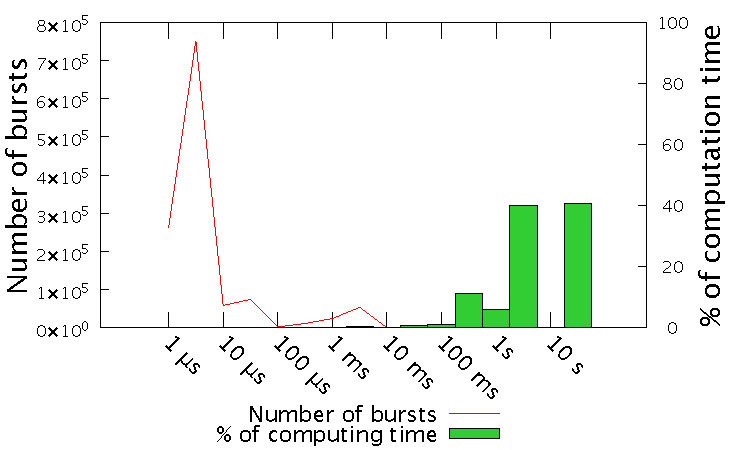
\includegraphics[width=1\columnwidth]{stats_plot/stats_plot.pdf}
  \caption{Bursts histogram produced by \texttt{stats} tool}
  \label{fig:stats_plot}
\end{figure}

With respect to the normalizations, we provide the possibility of applying
first a logarithmic normalization, useful when the parameter range is wide
and can bias the results of the cluster analysis. The logarithmic 
normalization can be applied to each parameter independently. The second 
normalization is a pure range normalization to set the parameter values 
in range $[0,1]$, following the formula  range 
($\forall a_{i}\in A,a_{i}\leftarrow(a_{i}-min(A))/(max(A)-min(A))$).
When using the range normalization, it will be applied to each parameter used,
so as to guarantee that all of them have the same weight in the analysis. If
we to add more weight one of the parameters used in the cluster analysis, we
can apply a multiplicative factor.

To clarify how the different normalizations and filters work, this is the 
order as they are applied: when a CPU burst is read, its duration is checked
and then the different parameters that have range filters defined; to those
bursts that pass the filters its performed the logarithmic normalization of 
each parameter that requires it and afterwards the range normalization. 
Finally, the scaling factor is applied.

\subsubsection*{3. Select the output plots}

We can combine the parameters defined previous to generate GNUplot scripts
of 2D and 3D scatter-plots. The plots can print both the normalized data or
the raw data (before normalizations). The user can tune tune the ranges to 
print and also the axis-labels of the plots. In addition, users can let the
library to produce all 2D plots obtained combining all metrics defined.

Once having the parameters, filters and plots, we can run the application
\texttt{Clustering\-DataExtractor} to extract the data and produce the plots 
described before runing the cluster algorithm. The resulting plots will 
show all the data available, distinguishing between the duration filtered 
bursts, the range filtered bursts and the ones that will take part in the 
cluster analyses. These plots are an useful aid to fine tune the parameter 
filters and normalizations.

\subsubsection*{4. Select the cluster algorithm}

Even though the Aggregative Cluster Refinement and DBSCAN are the two basic
algorithms offered by the \texttt{ClusteringSuite} package, there is a few
more clustering algorithms offered to the user. Table~\ref{tab:cluster_algorithms}
contains the list of these algorithms and their parameters. It is interesting
to note that the Aggregative Cluster Refinement is the only algorithm that
does not require any parameter and it not have to be expressed in the
XML configuration file.

\begin{table}
  \centering
  
  \caption{Cluster algorithms included in the \texttt{libClustering} and their
  parameters}
  \label{tab:cluster_algorithms}
  
  \begin{tikzpicture}
  \node [fill=figureshade,rounded corners=5pt]
  {
  
  \vspace{10pt}
  
  \ra{1.3}
  
  \begin{threeparttable}[b]
  
  \begin{tabular}{@{}*>{\tt}l>{\tt}^l@{}}
  \toprule
  \bf Cluster Algorithm Name  & \bf Parameters \\
  \midrule
  DBSCAN                  & epsilon, min\_points \\
  GMEANS                  & critical\_value, max\_clusters \\
  CAPEK\tnote{1}          & k \\
  MUSTER\_PAM\tnote{1}    & max\_clusters \\
  MUSTER\_XCLARA\tnote{1} & max\_clusters \\
  
  \bottomrule

  \end{tabular}
  
  \begin{tablenotes}
    \item[1] \texttt{libClustering} includes a common interface to this
    algorithms offered by the MUSTER library (\url{http://tgamblin.github.com/muster/main.html}
  \end{tablenotes}
  
  \end{threeparttable}
  
  };
  \end{tikzpicture}
  
\end{table}

For further information about the different algorithms included in the
package, we point to the following papers: \cite{Ester:KDD96} for DBSCAN 
algorithm, \cite{Foina:Multicore2010} for GMEANS and \cite{Gamblin:ICS10} for
CAPEK, PAM and XCLARA.

In case of DBSCAN we provide the application \texttt{DBSCANParametersApproximation}
to help the paremeter selection, according to the technique described
in~\cite{Ester:KDD96}.

\begin{table}
  \centering
  
  \caption{\texttt{BurstClustering} tool parameters}
  \label{tab:burstclustering_params}
  
  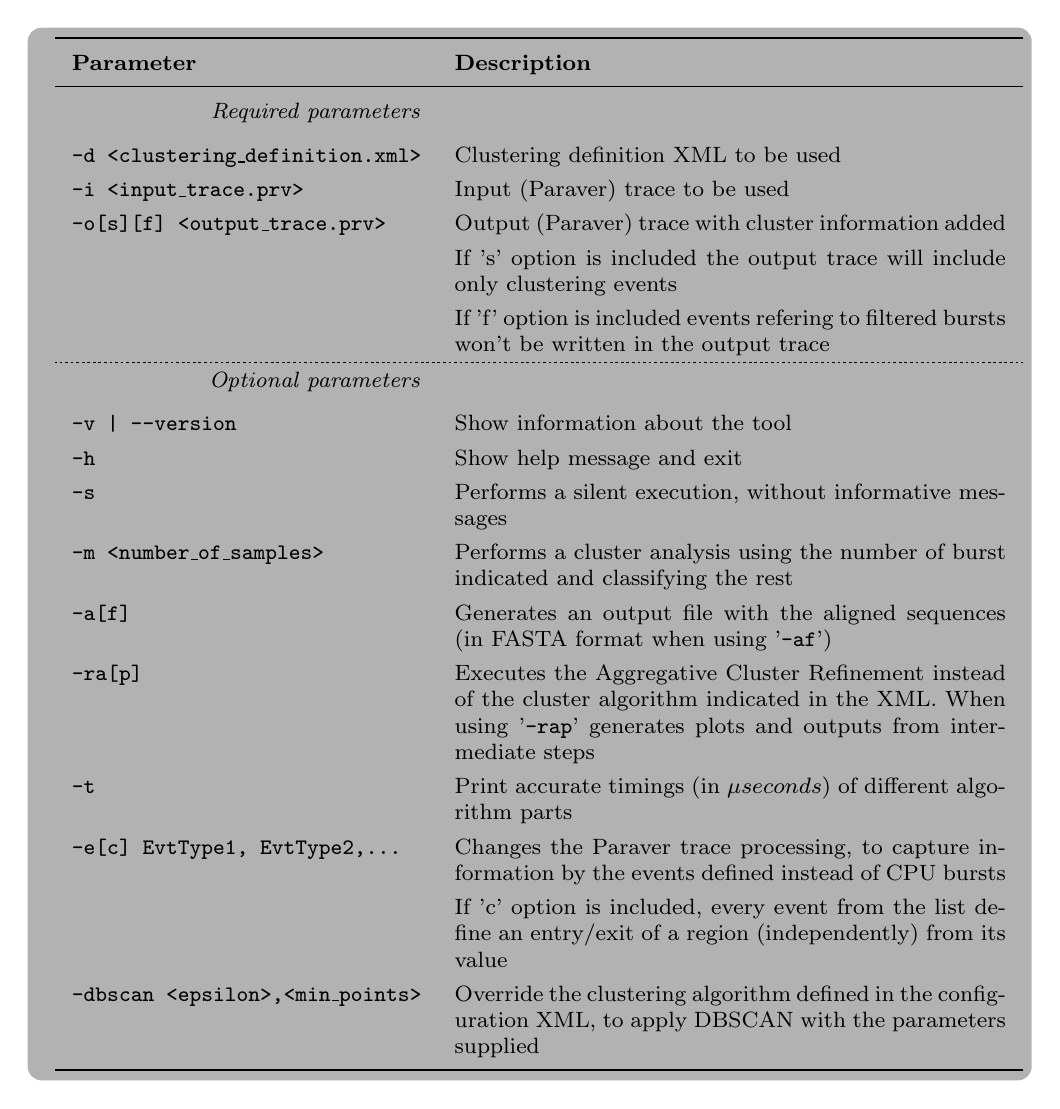
\begin{tikzpicture}
  \node [fill=figureshade,rounded corners=5pt]
  {
  
  \vspace{10pt}
  
  \ra{1.3}
  \footnotesize
  
  \begin{tabular}{>{\tt}lp{7cm}}
  \toprule
  \bf Parameter                   & \bf Description \\
  \midrule
  \multicolumn{1}{r}{\textit{Required parameters}} \\[1ex]
  -d <clustering\_definition.xml>  & Clustering definition XML to be used \\
  -i <input\_trace.prv>            & Input (Paraver) trace to be used \\
  -o[s][f] <output\_trace.prv>     & Output (Paraver) trace with cluster information added \\
				   & If 's' option is included the output trace will include only clustering events \\
				   & If 'f' option is included events refering to filtered bursts won't be written in the output trace \\
  \hdashline[1pt/1pt]
  \multicolumn{1}{r}{\textit{Optional parameters}} \\[1ex]
  -v | --version		  & Show information about the tool \\
  -h                              & Show help message and exit \\
  -s                              & Performs a silent execution, without informative messages \\  
  -m <number\_of\_samples>        & Performs a cluster analysis using the number of burst indicated and classifying the rest \\
  -a[f]                           & Generates an output file with the aligned sequences (in FASTA format when using '\texttt{-af}') \\
  -ra[p]                          & Executes the Aggregative Cluster Refinement instead of 
                                    the cluster algorithm indicated in the XML. When using
                                    '\texttt{-rap}' generates plots and outputs from
                                    intermediate steps \\
  -t                              & Print accurate timings (in $\mu seconds$) of different algorithm parts \\
  -e[c] EvtType1, EvtType2,...    & Changes the Paraver trace processing, to capture information by the events defined instead of CPU bursts \\
				  & If 'c' option is included, every event from the list define an entry/exit of a region (independently) from its value \\
  -dbscan <epsilon>,<min\_points> & Override the clustering algorithm defined in the configuration XML, to apply DBSCAN with the parameters supplied \\

  \bottomrule

  \end{tabular}
  
  };
  \end{tikzpicture}
  
\end{table}

\subsubsection*{5. Execute the cluster analysis}

Once defined the different elements necessary to perform the analysis, we
need to execute the \texttt{BurstClustering} tool. The different parameters 
of this tool and a short description of them are listed in 
Table~\ref{tab:burstclustering_params}. Basically, to perform a regular 
analysis using the cluster algorithm defined in the XML file we need to 
execute the command:

\begin{figure}[!h]
  
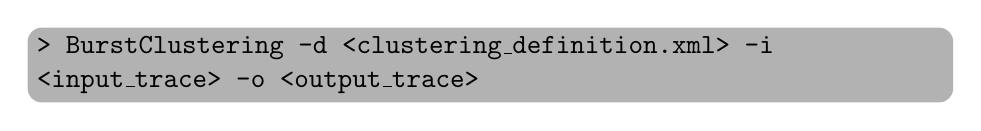
\begin{tikzpicture}
\node [fill=figureshade,rounded corners=5pt]
{

\begin{minipage}{.95\textwidth}

\texttt{> BurstClustering -d <clustering\_definition.xml> -i <input\_trace> -o <output\_trace>}

\end{minipage}
};
\end{tikzpicture}

\end{figure}

The tool will process the information provided in the configuration file,
extract the data from the input trace, execute the cluster algorithm and then
generate the required output plots, extrapolation files and the output trace.
These files will be explained in the further step.

In case we want to execute the Aggregative Cluster Refinement algorithm, the
command varies slightly:

\begin{figure}[!h]
  
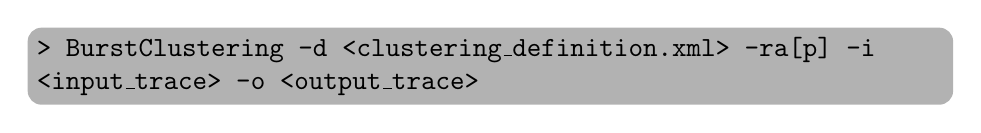
\begin{tikzpicture}
\node [fill=figureshade,rounded corners=5pt]
{

\begin{minipage}{.95\textwidth}
\texttt{> BurstClustering -d <clustering\_definition.xml> -ra[p] -i <input\_trace> -o <output\_trace>}
\end{minipage}
};
\end{tikzpicture}

\end{figure}

By adding the \texttt{-ra} parameter, the tool discards the algorithm
indicated in the clustering definition XML file and then applies this
different algorithm. In case we use the parameter \texttt{-rap}, the tool
will produce, apart from the regular outputs, the traces and plots of 
intermediate steps of the Aggregative Cluster Refinement algorithm.

\subsubsection*{6. \texttt{BurstClustering} tool outputs}

The \texttt{BurstClustering} offers three main outputs: scatter-plots of
the different metrics, a cluster statistics file (including the extrapolation)
and a reconstructed Paraver trace. In addition, it also generates the
refinement tree, when using the Aggregative Cluster Refinement. Optionally,
it can produce the a file with the sequence alignment and a file containing
the Cluster Sequence Score values. Here we will describe briefly all of them.

The \textbf{scatter-plots} are simply GNUplot scripts that can be load using
this plotting tool. As seen in previous steps, they can be 2 or 3 dimensional
combinations of different metrics used to characterize the CPU bursts. In any
case, the points in the scatter plots are coloured to distinguish the
different clusters found. These plots are useful to observe, qualitatively,
variations in the clusters with respect to the metrics used. In 
Figure~\ref{fig:plots_example} we show 4 different plots combining 8 different
hardware counters. First plot, \ref{subfig:plot_inst_ipc}, show the metrics
used by the cluster algorithm. In the rest of combinations we can observe that 
the clusters represent clear isolated clouds, with a minor exception of
the plot comparing Main Memory Accesses vs. L2 Data Cache Accesses,
\ref{subfig:plot_mainmem_l2}, where Cluster 4 (in red) appear in two different
clouds.

The plot scripts are named using the output trace prefix plus a trailing
string expressing the combination of metrics used. They have the extension
\texttt{.gnuplot}. All of them use a file ended in \texttt{.DATA.csv} that
contain on each line the different parameters described in the XML file plus 
the cluster identifier assigned for each CPU burst analysed.

\begin{figure}
  \centering
  \begin{tabular}{|c|c|}
  
  \subfloat[Instructions vs. IPC]
  {
    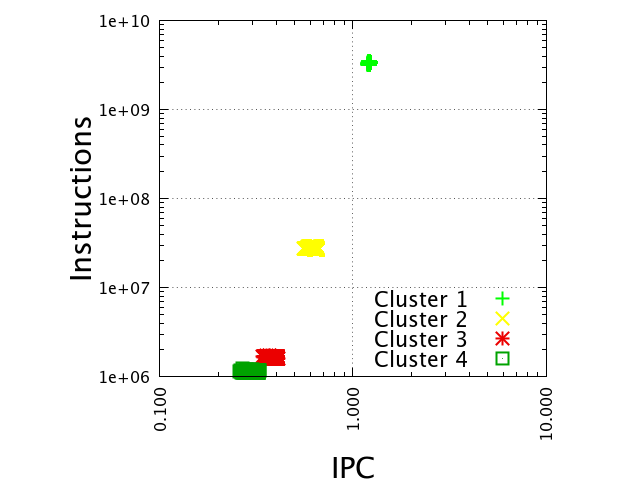
\includegraphics[width=.45\columnwidth]{plots_example/inst_vs_ipc_plot.png}
    \label{subfig:plot_inst_ipc}
  }
  &
  \subfloat[Stores vs. Loads]
  {
    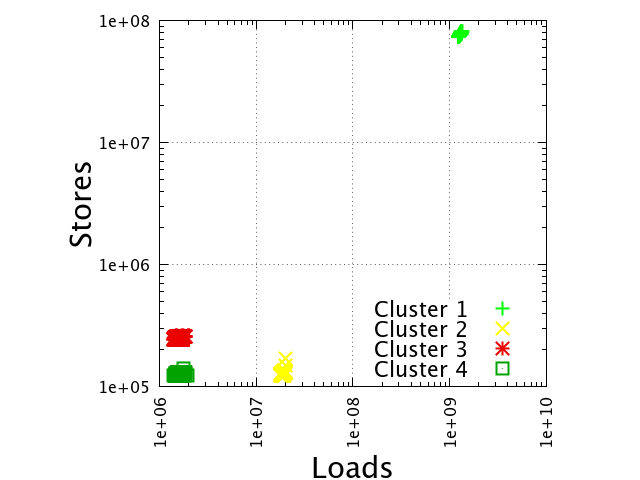
\includegraphics[width=.45\columnwidth]{plots_example/stores_vs_loads_plot.png} 
  }
  \\
  \subfloat[Main memory accesses vs. L2 data cache acessess]
  {
    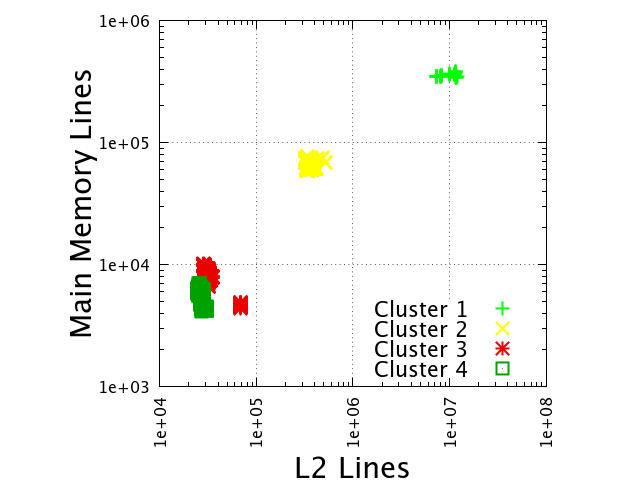
\includegraphics[width=.45\columnwidth]{plots_example/mainmem_vs_l2_plot.png}
    \label{subfig:plot_mainmem_l2}
  }
  &
  \subfloat[Integer instructions vs. Floating point instructions]
  {
    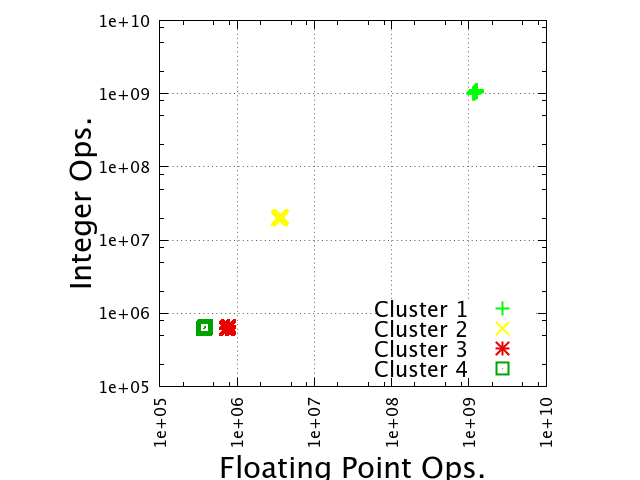
\includegraphics[width=.45\columnwidth]{plots_example/int_vs_fop_plot.png}
  }
  \\
  \end{tabular}
  
  \caption{Output plots produced by \texttt{BurstClustering} tool combining
  different metrics}
  \label{fig:plots_example}
  
\end{figure}

The \textbf{clustering statistics} file is a CSV file that contains the number
of individuals, the aggregated duration and the average duration per CPU 
burst, and the average values of extrapolation parameters defined in XML,
for each cluster found. This file is really useful to analysed quantitatively
the behaviour of the different clusters found. The clusters statistics file 
is named using the prefix of the input trace, but ending in 
\texttt{.clusters\_info.csv}.

% As an example, we provide a spreadsheet where
% we can import the statistics from a set of native performance counters of
% the Power PC 970 processor, ant it will compute a really useful CPU 
% breakdown model for each cluster.

Next output that is always produced is the \textbf{output trace}. Basically,
this is exactly the same input trace where all the CPU burst have been
surrounded using a certain events to identify them. Thanks to these events, we
can take advantage of the vast analysis power of Paraver and Dimemas to 
perform further analyses and correlate the clusters with all the information
present on the trace. For example, we can observe the time-line distribution 
of the different computation regions detected. An example of Paraver 
time-line and its corresponding duration profile can be seen in 
Figure~\ref{fig:paraver_clustering}. We provide a set of Paraver configuration
files with pre-defined views and histograms related to cluster events.

\begin{figure}
  \centering
  \subfloat[Time-line distribution of discovered clusters]
  {
    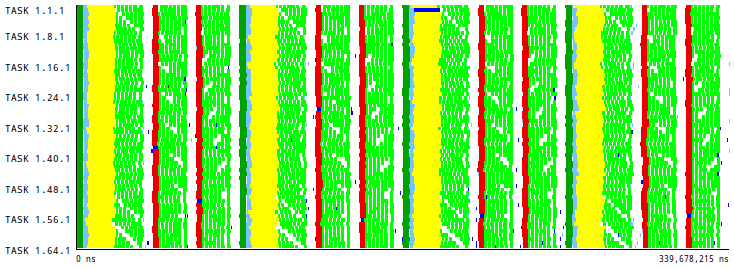
\includegraphics[width=1\columnwidth]{paraver_example/paraver_clusters_timeline.png}
  }
  
  \subfloat[Duration histogram of the clusters per application task]
  {
    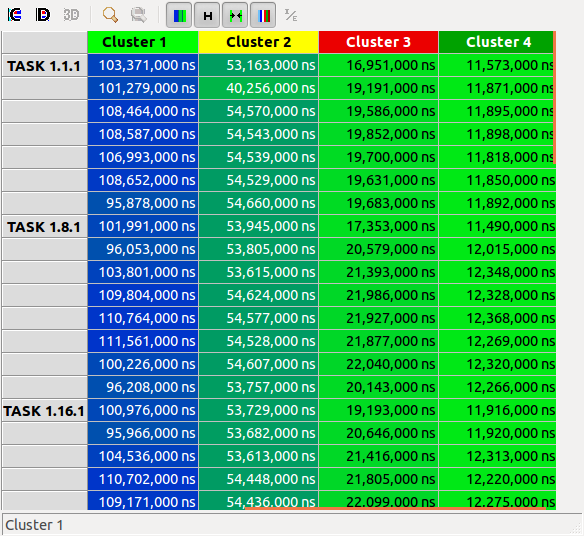
\includegraphics[width=.8\columnwidth]{paraver_example/paraver_clusters_profile.png}
  }
  
  \caption{A Paraver time-line and profile showing information related
  to a cluster analysis}
  \label{fig:paraver_clustering}
\end{figure}

In case we executed the Aggregative Cluster Refinement algorithm, the tool
will also produce a \textbf{refinement tree} file. This file has the same 
prefix as the output trace and the extension \texttt{TREE.dot}. It is a
text file that describes the refinement tree using the DOT language. To
visualize it we require the GraphViz\footnote{\url{http://www.graphviz.org/}}
software package. We also recommend using of the interactive tool 
\texttt{xdot}\footnote{\url{http://code.google.com/p/jrfonseca/wiki/XDot}}
to navigate through the refinement tree output. An example of a refinement
tree can be seen in Figure~\ref{fig:refinement_tree}.

\begin{sidewaysfigure}[!htp]
  
  \centering
  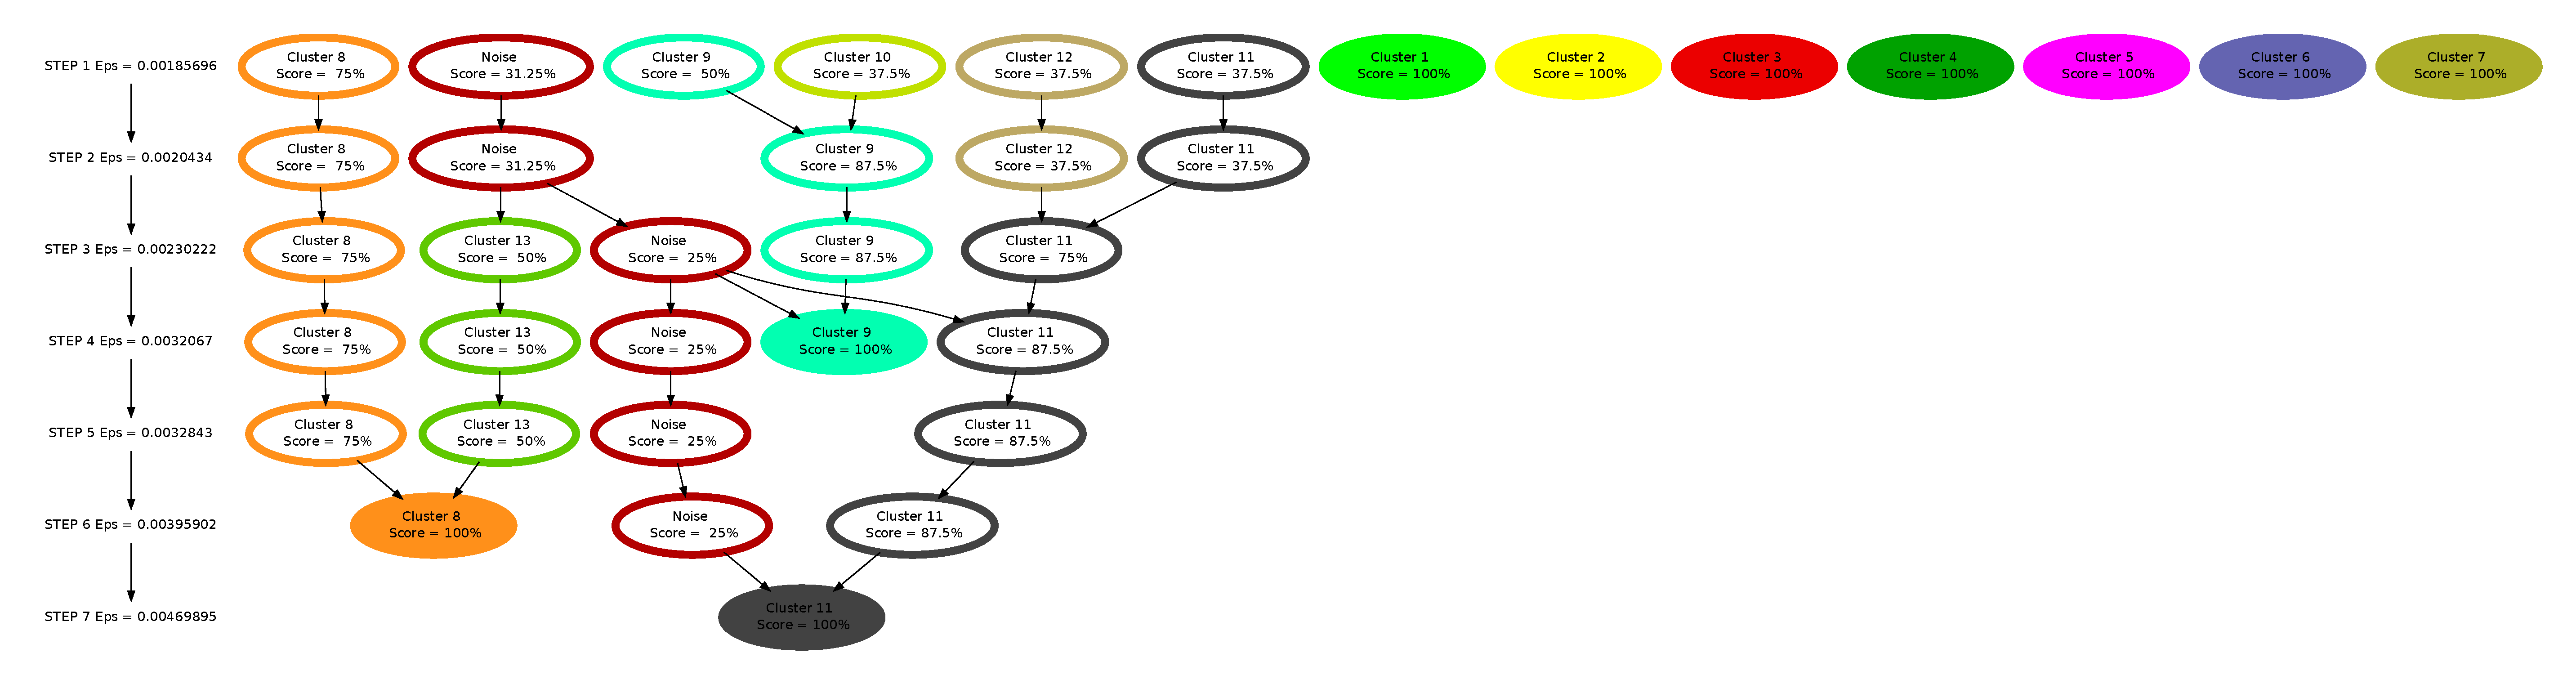
\includegraphics[width=1\columnwidth]{refinement_tree/refinement_tree.pdf}
  \caption{Example of a refinement tree produced by \texttt{BurstClustering} tool}
  \label{fig:refinement_tree}

\end{sidewaysfigure}

Finally, using the parameter \texttt{-a}, the tool will produce a CSV file
containing the sequences obtained after applying the Cluster Sequence Score.
This file, named as the output trace with the extension \texttt{.seq}, contains
the sequence of the cluster identifiers (numbers) and gaps (marked as hyphens)
introduced by the alignment algorithm for each task and thread present on
the input trace. If use the parameter \texttt{-af}, the file will be generated
in the FASTA format, transforming the first 21 clusters in an amino-acid 
identifier. The FASTA file can be load in any alignment software, such
as ClustalX\footnote{\url{http://www.clustal.org/}} for its visualization. In
Figure \ref{fig:clustalx_example} we can see a ClustalX window with a set of
aligned sequences.

If we use any of these two last parameters, the tool will also produce a file
with the extension \texttt{SCORES.csv}, that contains the numerical results of
the Cluster Sequence Score. 

\begin{figure}
  \centering
  
  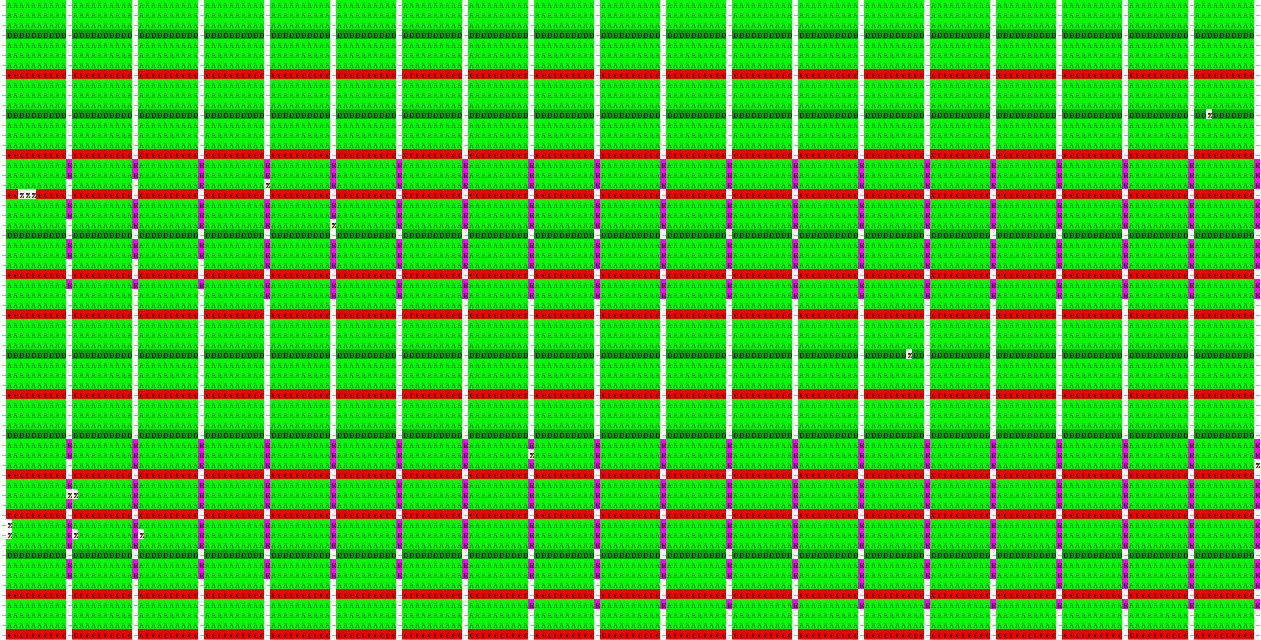
\includegraphics[width=1\columnwidth]{sequences_example/sequences_clustalx.png}
 
  \caption{ClustalX sequence alignment window}
  \label{fig:clustalx_example}
\end{figure}


When using the Aggregative Cluster Refinement with the parameter \texttt{-rap}
the tool will produce the plots, traces, refinement trees, sequence files
and score files for each refinement step. The intermediate statistics files
will not be generated and these intermediate trace files will only contain
cluster events, to check the intermediate cluster distribution, but not to
correlate them with other information. The intermediate files will have an
inter-fix \texttt{STEPX} in their file name, to distinguish at which step
(iteration) of refinement were produced.

Finally, it is interesting to note that we guarantee the colour coherence
in all those outputs generated by the \texttt{BurstClustering} that use colour 
information to distinguish the cluster identifiers. In case of ClustalX we 
provide a modified version of software package with the required amino-acid
colouring.


\chapter{Creating the clustering definition XML}
\label{chap:xml_definition}

In this chapter we deeply describe the structure of the clustering definition
XML.

\section{Clustering definition XML description}

In brief, the clustering definition XML file contains the description of four
elements of the clustering process: the parameters associated to each CPU burst
in the trace used by cluster analysis and the extrapolation process; the
filtering ranges and normalizations applied to this data; the cluster 
algorithm to be used; and finally, the description of the different output
plots, generated as GNUplot scripts. We can see how these different parts are
distributed in the XML file in Figure \ref{fig:xml_structure}.

Following the current description of the file it could be easily generated
using a regular text editor or a XML editor.

% In the current
% \texttt{ClusteringSuite} package, there is no an specific application to 
% generate it, but it is planned for future versions.


\begin{figure}
  \centering
  
  \begin{tikzpicture}
  \node [fill=figureshade,rounded corners=5pt]
  {
    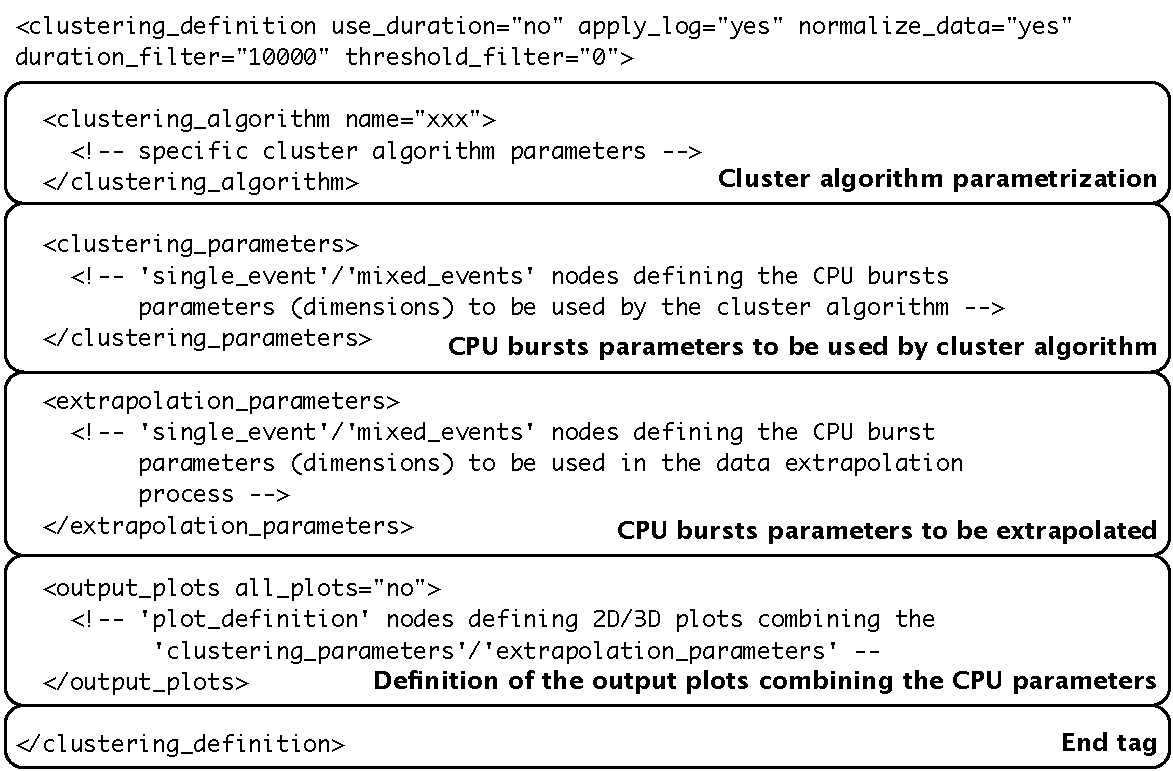
\includegraphics[width=1\columnwidth]{clustering_xml/xml_structure.pdf}
  };
  \end{tikzpicture}
  
  \caption{Clustering definition XML file structure}
  \label{fig:xml_structure}
  
\end{figure}

\section{Parameter selection}

There are two ways to define how the parameters are read from a Paraver trace.
First, the values of individual events situated at the end of the Running 
State, using \texttt{single\_event} nodes. Second, combining the values of
two different events with a basic mathematical operation, using 
\texttt{mixed\_events} nodes.

A \textbf{\texttt{single\_event}} node, see Figure~\ref{subfig:xml_single_event},
contains first two attributes: \texttt{apply\_log} that indicates if
a logarithmic normalization will be applied to its values; the \texttt{name}
parameter is the label the will be used in the different output file. 
The inner node \texttt{event\_type} is mandatory, to define the event type 
that appears in the Paraver trace. Optional nodes \texttt{range\_min} and 
\texttt{range\_max} are used to filter the CPU burst outside these 
boundaries. Finally, optional node \texttt{factor} is a multiplicative
value so as to weight the parameter value.

A \textbf{\texttt{mixed\_events}} node, see Figure~\ref{subfig:xml_mixed_events},
is pretty similar to the previous one, but includes two mandatory internal
nodes \texttt{event\_type\_a} and \texttt{event\_type\_b}, to define the
two types of events involved, and the attribute \texttt{operation} to define
the mathematical operation applied to the values read. Possible operations
are \texttt{+}, \texttt{-}, \texttt{*} and \texttt{/}. The operation is 
applied to the values of the two events defined, \textit{before} the 
logarithmic normalization.

To define the CPU bursts parameters that will be used by the cluster algorithm,
they have to be placed below the \texttt{clustering\_parameters} node,
see Figure~\ref{fig:xml_structure}. To define those that will be used to
characterize the resulting clusters (as averages in the \texttt{.clusters\_info.csv}
file), we have to place them below the \texttt{extrapolation\_parameters} node.

If we want to use the duration of the CPU bursts as a parameter, we need to 
set to \textit{yes} the attribute \texttt{use\_duration} present in the root
node (\texttt{cluste\-ring\_definition}).

% The duration will always be used as
% parameter used by the cluster algorithm.

\begin{figure}
  \centering
  
  \subfloat[\texttt{single\_event} node structure]
  {
    \begin{tikzpicture}
    \node [fill=figureshade,rounded corners=5pt]
    {
    \includegraphics[scale=.7]{clustering_xml/xml_single_event_definition.pdf}
    };
    \end{tikzpicture}
    \label{subfig:xml_single_event}
  }
  
  \subfloat[\texttt{mixed\_events} node structure]
  {
    \begin{tikzpicture}
    \node [fill=figureshade,rounded corners=5pt]
    {
    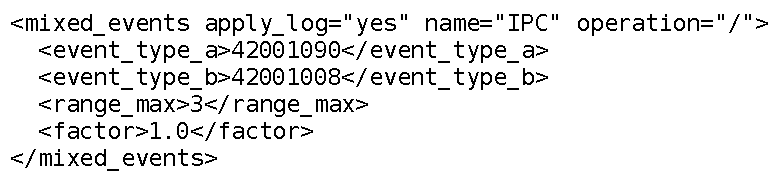
\includegraphics[scale=.7]{clustering_xml/xml_mixed_events_definition.pdf}
    };
    \end{tikzpicture}
    \label{subfig:xml_mixed_events}
  }
  
  \caption{Nodes to define the parameters extracted from a trace}
  \label{fig:xml_events_definition}

\end{figure}

\subsubsection{Filtering and normalization}

The filtering and normalization is expressed at two points of the XML file.
We have seen that the parameter definition nodes include both a range 
filtering and also a logarithmic normalization. The filtering information
included in the extrapolation parameters is not taken into account.

The second point is the root node. In this node we find different attributes,
see Figure~\ref{fig:xml_structure} regarding filters and normalizations.
First one is \texttt{apply\_log}, that indicates if logarithmic normalization
will be applied to the burst duration, if used. Next one is \texttt{normalize\_data},
that indicates if a final range normalization will be applied to the values 
of \textit{all} parameters (independently). Next we find the
\texttt{duration\_filter} to discard those burst with less duration than the 
indicated~\footnote{The default units for this field are microseconds, but you can
change them adding 'D' for days, 'M' for minutes, 'H' for hours, 's' o 'S' for
seconds, 'm' for miliseconds and 'n' for nanoseconds following the value
you insert}. Finally, the \texttt{threshold\_filter} is a percentage to discard
all the clusters found whose aggregated duration represents less percentage of
the total clusters duration than the indicated.

\subsubsection{Output plots}

Once defined the parameters used to characterize the CPU bursts, below
the \texttt{output\_plots} node we can define the output plots combining
the different metrics.

If we set the attribute \texttt{all\_plots} of this main node to \textit{yes},
the \texttt{libTrace\-Clustering} library will generate all possible 2D plots
combining the parameters defined (clustering parameters and extrapolation
parameters). If we want to manually define the combinations we can use 
the \texttt{plot\_definition} structure, see Figure \ref{fig:xml_plot_definition}.

What we find first in the \texttt{plot\_definition} node is the attribute
\texttt{raw\_metrics}. In case we applied normalization to the clustering
parameters setting this attribute to ``yes'' indicates that the resulting
plot will use the raw values of the parameters. Then we find three kind
of nodes \texttt{[x|y|z]\_metric}. Each of these nodes has a mandatory
attribute \texttt{title} that will be used as the plot label for the
corresponding axis. They have two optional attributes \texttt{max} and
\texttt{min} to define the axis range. Finally, the content of each of
these nodes must be the \textit{name} attribute of any of the parameters 
defined previously (clustering parameter of extrapolation parameter). In case
we want to use the duration, as it is defined differently from regular
parameters, it has to be referenced simply using the text \texttt{Duration}.

We can combine up to three metrics to create a 3 dimensional scatter-plot,
where the individuals will be distinguished in series according to the
cluster identifier assigned. The same is applicable when using just two
metrics (\textit{x} and \textit{y}). If we just define a single metric 
(\textit{x metric}), the resulting plot will be a 2 dimensional plot using
the cluster identifier as y axis.

\begin{figure}
  \centering
  \begin{tikzpicture}
  \node [fill=figureshade,rounded corners=5pt]
  {
  \includegraphics[scale=.7]{clustering_xml/xml_plot_definition.pdf}
  };
  \end{tikzpicture}
  \caption{\texttt{plot\_definition} node of the clustering defintion XML}
  \label{fig:xml_plot_definition}
\end{figure}

\bibliographystyle{plain} % Title is link if provided
% \bibliography{papers_db}
\bibliography{cluster_analysis_thesis_bibliography}
\addcontentsline{toc}{chapter}{Bibliography}


\end{document}